\chapter{Background}
\label{ch:Background}

\section{Mathematical}
\subsection{Mathematical Representations of 3D Orientations}
Rotations can be expressed in several ways, I will briefly describe the ones used in this thesis.

\subsubsection{Rotation matrix}
A rotation matrix \mtf{b}{a} $\in \mathbb{R}^{3\times3}$ transforms an arbitrary vector from the coordinate system $\mathcal{B}$ to the coordinate system $\mathcal{A}$.\\
\dots\\
Rotation matrices can be concatenated, but this must be done in reverse order, e.g.
\begin{equation}
	{}_\mathcal{C}\vb{p} = \mtf{c}{a}{}_\mathcal{A}\vb{p} = \mtf{b}{c}\mtf{a}{b}{}_\mathcal{A}\vb{p}
\end{equation}
to transform the point ${}_\mathcal{A}\vb{p}$ over the intermediate frame $\mathcal{B}$ to the coordinate system $\mathcal{C}$.

\subsubsection{Euler angles}
Euler angles are the closest to intuition but mathematically the worst way to represent orientations.
Every orientation can be produced by a concatenation of three rotations around each of the coordinate axes.
Because the resulting orientation depends on the order of which the rotations were performed, there are different conventions.
Furthermore the conventions can be divided into intrinsic and extrinsic.
Intrinsic rotation means that the coordinate system moves with the moving object, whereas with extrinsic rotations the original coordinate system remains static.
The most common convention is the zyx (intrinsic I think?) (first rotation around z-axis and last around x-axis), where the angles are called yaw, pitch and roll.\\
The disadvantages are the many conventions and the possibility of singularity.

\subsubsection{Quaternions}
wow
\begin{equation}
	\vb{q} = a + b\vb{i} + c\vb{j} + d\vb{k}
\end{equation}
with
\begin{equation}
	\vb{i}^2 = \vb{j}^2 = \vb{k}^2 = \vb{i}\vb{j}\vb{k} = -1
\end{equation}
\itodo{Improve quaternion text and add new stuff}
\begin{equation}
	\alpha \in[0, \pi] @ \mathbf{j} \underbrace{\left[j_{x}, j_{y}, j_{z}\right]^{\top}}_{\|j\|_{2}=1}
	\quad\cong\quad {}^{\mathcal{B}}_{\mathcal{A}} q
	=\cos \left(\frac{\alpha}{2}\right)+\left(j_{x} \mathbf{i}+j_{y} \mathbf{j}+j_{z} \mathbf{k}\right) \sin \left(\frac{\alpha}{2}\right)
	\end{equation}
The quaternion can then be calculated with
\begin{equation}
	\vb{q} =
	\begin{bmatrix}
		\cos(\frac{\alpha}{2})\\
		\vb{j}\vdot\sin(\frac{\alpha}{2})
	\end{bmatrix}
\end{equation}

\subsection{Vector projection}
\label{subsec:vector_projection}
In general, the rotation to align a vector $\vb{v}_1$ with a vector $\vb{v}_2$ can be expressed using a quaternion.
At first both vectors must be normalized, resulting in the two unit vectors $\vu{v}_1$ and $\vu{v}_2$.
The rotation axis is perpendicular to both vectors and can thus be calculated using the cross product
\begin{equation}
    \vb{j} = \frac{\vu{v}_1 \cp \vu{v}_2}{\norm{\vu{v}_1 \cp \vu{v}_2}}.
\end{equation}
The angle between two vectors can be calculated with
\begin{equation}
    \cos(\alpha) = \frac{\vu{v}_1 \vdot \vu{v}_2}{\norm{\vu{v}_1} \cdot \norm{\vu{v}_2}}
    = \vu{v}_1 \vdot \vu{v}_2 \implies
    \alpha = \arccos(\vu{v}_1 \vdot \vu{v}_2).
\end{equation}
The denominator is equal to 1 (because the norm of an unit vector is 1) and thus omitted.



\section{Sensors}
\subsection{\glsentrytext{imu}}
An \gls{imu} is used to track the orientation and position of an object.
Common uses are in the aerospace or automotive industry, often in combination with other sensors, to give information about the pose and position of a vehicle.
More recently with the invention of \gls{mems} and specifically \gls{mems}-\gls{imu}s which allow for a very small form factor at a low cost, \gls{imu}s are also used in consumer electronics such as smartphones or fitness tracker.
An \gls{imu} usually consists of the three following sensors.
The acceleration is measured using an accelerometer and can be used to determine the velocity and the covered distance by integrating the acceleration with respect to time once respectively twice.
The gyroscope gives information about the change of orientation.
The third part is the magnetometer, which is able to measure the earth's magnetic field and is used to correct the measurements of the gyroscope.
It allows for the determination of the absolute heading, whereas the gyroscope can only measure relative change. But because it is very sensitive to other magnetic objects, it is often omitted.
\gls{imu}s can be typically divided into the two following categories.\\
\begin{figure}[htbp]
	\centering
	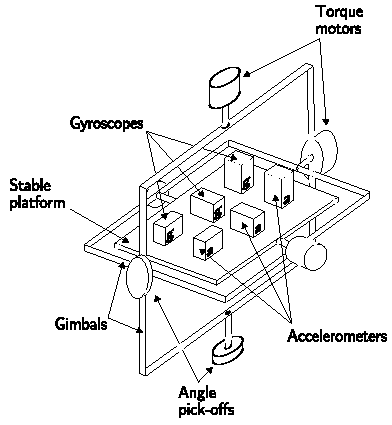
\includegraphics[width=0.4\linewidth]{stable_platform_imu}
	\caption{A stable platform \acrshort{imu} \cite{Woodman2007}}
	\label{fig:stable_platform_imu}
\end{figure}
In the first type, the stable platform systems, the inertial sensors are mounted in such way, that they are always aligned with the reference frame.
This is achieved using gimbals, which allow movement along all three axes.
The gyroscopes on the platform measure the rotation and send them to torque motors, which rotate the gimbals to keep the platform in alignment with the reference frame.
A typical setup of a stable platform system can be seen in fig. \ref{fig:stable_platform_imu}.
The advantage of stable platform systems is that the calculation of orientation and position is straight forward.
The angles of the gimbals can be measured to get the orientation and to get the position, the accelerometer measurements have to be be corrected for gravity and be integrated two times.
No coordinate transformation is necessary.
The disadvantages are that the mechanical structure of the setup is complex, needs regular maintenance, requires a lot of space and has high costs.\\
The second type are strapdown systems, which are mostly used today.
As the name suggests all the parts are fixed onto the device and are thus not anymore always aligned with the reference frame.
Advantages are that due to the lack of gimbals and motors a significantly smaller build is possible while also being cheaper to mass produce.
A disadvantage is that the calculation of the orientation and position is more complex, the rate gyroscopes have to be integrated to get the orientation and can then be used to transform the accelerometer signals into the reference frame.
But with the decrease of computational cost this disadvantages continues to diminish.\\
There are many different types of gyroscopes and accelerometers such as mechanical, optical or solid state, but only the functionality of \gls{mems} will be described, because those will also be used in the experiment.
Information about the working principle of other systems and also much more information about \gls{imu}s in general can be found in \cite{Woodman2007}.\\
\gls{mems} consist of electrical and/or mechanical components in the size of \SI{100}{\nano\metre} to \SI{1}{\milli\metre}, allowing for a very small form factor.
Other characteristics of \gls{mems} are that they can easily be mass produced allowing for low cost and usually also need less power than traditional systems, because everything is integrated on the chip \cite{Shaeffer2013}.
Almost all consumer grade electronics uses \gls{mems}-\gls{imu}s nowadays, but they also find more and more use in many industry segments, as their accuracy continues to improve \cite{Perlmutter2016}.

\subsubsection{\glsentrytext{mems} Accelerometer}
\begin{figure}[htb]
	\centering
	\begin{subfigure}{0.48\textwidth}
		\centering
		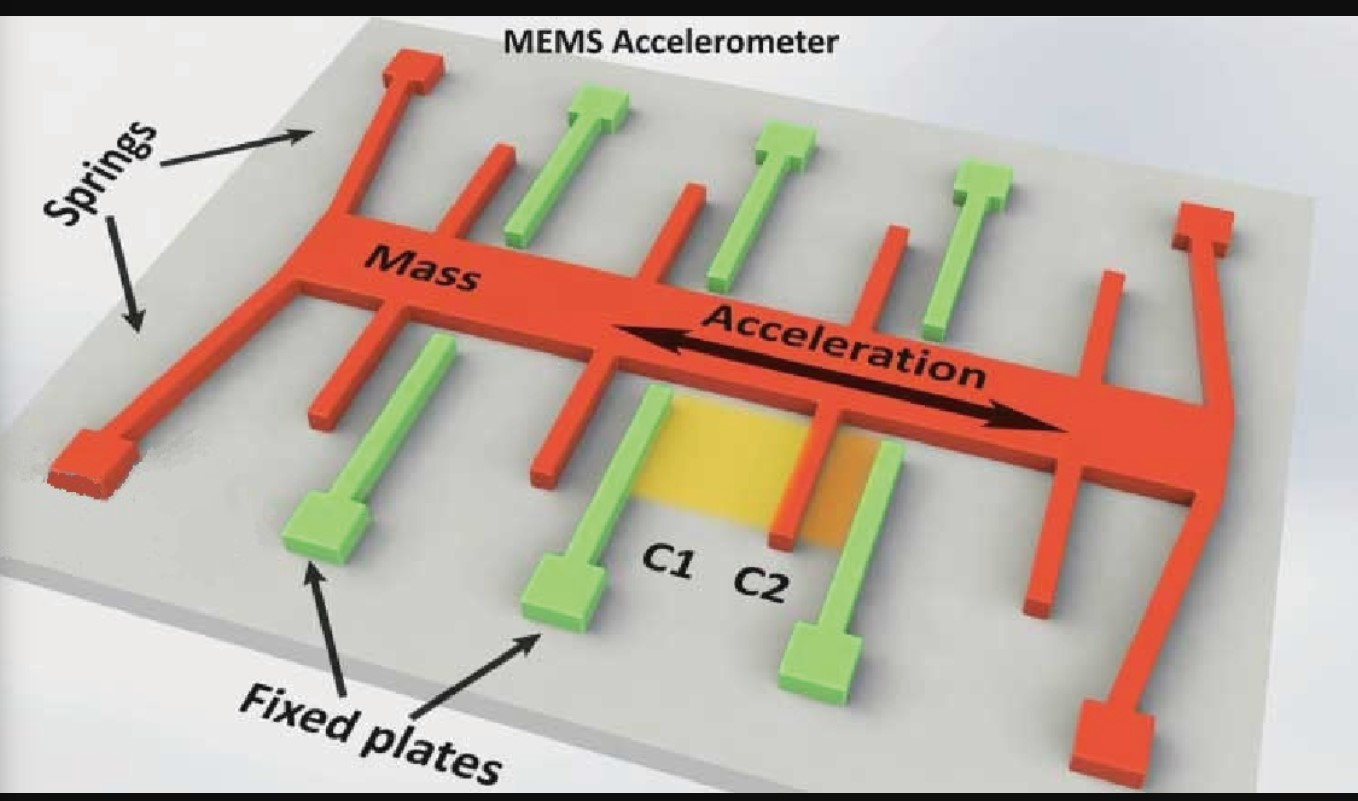
\includegraphics[width=\textwidth]{MEMS_Accelerometer}
		\caption{\acrshort{mems} accelerometer}
		\label{fig:MEMS_Accelerometer}
	\end{subfigure}
	% \hfill
	\begin{subfigure}{0.48\textwidth}
		\centering
		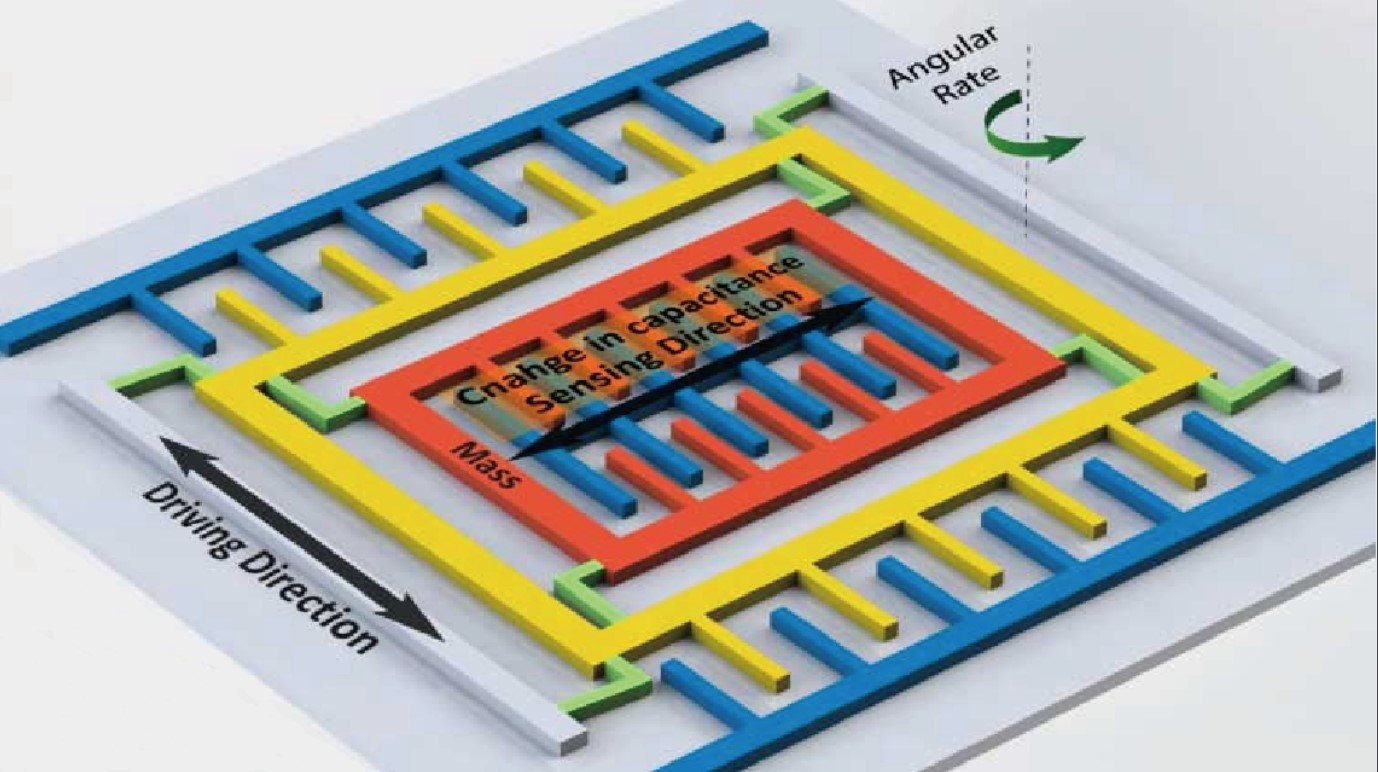
\includegraphics[width=\textwidth]{MEMS_Gyroscope}
		\caption{\acrshort{mems} gyroscope}
		\label{fig:MEMS_Gyroscope}
	\end{subfigure}
	\caption{Micro structure of \acrshort{mems} TODO: Better images}
	\label{fig:MEMS_design}
\end{figure}
The accelerometer is used to measure the acceleration.
Besides dynamic acceleration there is the static and constant gravity acceleration on earth, which is measured by the \gls{imu} in upward direction.
This allows for the determination of one axis of the \gls{imu}, even if it is not moving.
Often times only the dynamic accelerations are of interest and to get them the acceleration data during stand still must be measured and subtracted.
The micro structure of a \gls{mems} accelerometer is shown in figure \ref{fig:MEMS_Accelerometer}.
A mass is suspended by springs along one axis and if an acceleration along this axis occurs, the mass moves in the opposite direction due to Newton's second law.
The mass has little fingers perpendicular to the axis along which the movement occurs, which affect the capacity between the fixed plates.
The change of capacity and thus voltage can be measured, from which the acceleration can be calculated.
To be able to measure the acceleration along all three axis the same setup is used three times, perpendicular to each other.

\subsubsection{\glsentrytext{mems} Gyroscopes}
A gyroscope measures the angular velocity.
The setup of a \gls{mems} gyroscope is similar to that of a \gls{mems} accelerometer.
A proof mass is suspended on a frame and responds to an input force.
\gls{mems} gyroscopes make use of the Coriolis effect, which states that an rotating object with the angular velocity $w$ of mass $m$ and velocity $v$ experiences a force
\begin{equation}
	F_C = -2m(w\times v).
\end{equation}
To measure the effect, a mass is vibrating along one axis, which in turn is also suspended.
If the mass is oscillating along one axis and a rotation is applied, a second oscillation on the axis perpendicular to the rotation axis can be observed.
E.g.\ if the mass oscillates along the x-axis and a rotation around the z-axis is applied, a vibration along the y-axis can be observed.
By measuring the amplitude and phase of the secondary oscillation the absolute value and direction of the angular velocity can be calculated.
While \gls{mems} gyroscopes do not achieve the same accuracy as optical gyroscopes they offer many advantages such as smaller physical properties (weight and size), lower power consumption and startup time as well as a significantly lower cost.
\gls{mems} gyroscopes have replaced other gyroscope types in most areas, but in areas where the highest precision possible is necessary, typically in military industry, optical gyroscopes are still used today \cite{Perlmutter2016}.

\subsubsection{(\glsentrytext{mems}) Magnetometer}
A magnetometer measures the local magnetic field.
Most sensors work using the Hall effect.
A current is set to flow through a conductive plate.
Without the presence of a magnetic field the electrons flow in a straight line, but if a magnetic field is introduced the electrons do get deflected to one side.
The voltage between the two sides can then be measured, from which the strength and direction of the magnetic field can be determined.\\
Without any magnetic disturbances, the magnetometer measures a constant local magnetic field vector.
The vector points to magnetic North and can thus be used to determine the heading.
Because the magnitude of the earth's magnetic field is very low (\SIrange{25}{65}{\micro\tesla}), the magnetometer readings can easily be influenced by other objects \cite{Kok2016}.
The distortions can be divided into two categories: hard or soft iron.
Hard iron distortions are created by objects which actively produce a magnetic field, causing a permanent bias.
Soft iron disturbances are due to deflections or altercations of an existing magnetic field.
Both types of disturbances can be removed with a proper calibration if there position and orientation, relative to the sensor, stays the same \cite{Guo2008}.
Every time the sensor is placed in a (magnetically) new environment, a recalibration is necessary.

\subsubsection{Typical \glsentrytext{mems} errors}
The errors can be divided into two categories: systematic and stochastic errors \cite{Zhang2019}.
Systematic errors or also known as calibration errors are constant over time and can be eliminated by calibration.
Typical examples are bias (offset), scaling or axis misalignments.
Integrating a constant bias once or twice leads to a drift (error grows linearly with respect to time) or a second-order drift (error grows quadratically) respectively.
Hence the elimination of the bias is necessary to get reliable estimations of the orientation, velocity or position, which are calculated by integrating the angular velocity or the accelerometer measurements.\\
Stochastic errors change at every measurement and can be modeled using a statistical approach.
The turn-on bias is different every time the \gls{imu} is powered up, but can be eliminated after a rest period.
Errors due to temperature fluctuations influencing the measurements are also common, but because most \gls{imu}s are equipped with a temperature sensor, the introduced error can be eliminated.
Harder to correct is the introduced error due to thermo-mechanical noise, which is measured as white noise.
The integration of white noise leads than to a random walk.\\
Angle errors introduced by random walk are usually the hardest to correct and are the reason, why the measurements of the gyroscope can not be trusted over a long period of time \cite{Woodman2007}.


\subsection{\glsentrytext{lidar}}
\begin{figure}[htb]
	\centering
	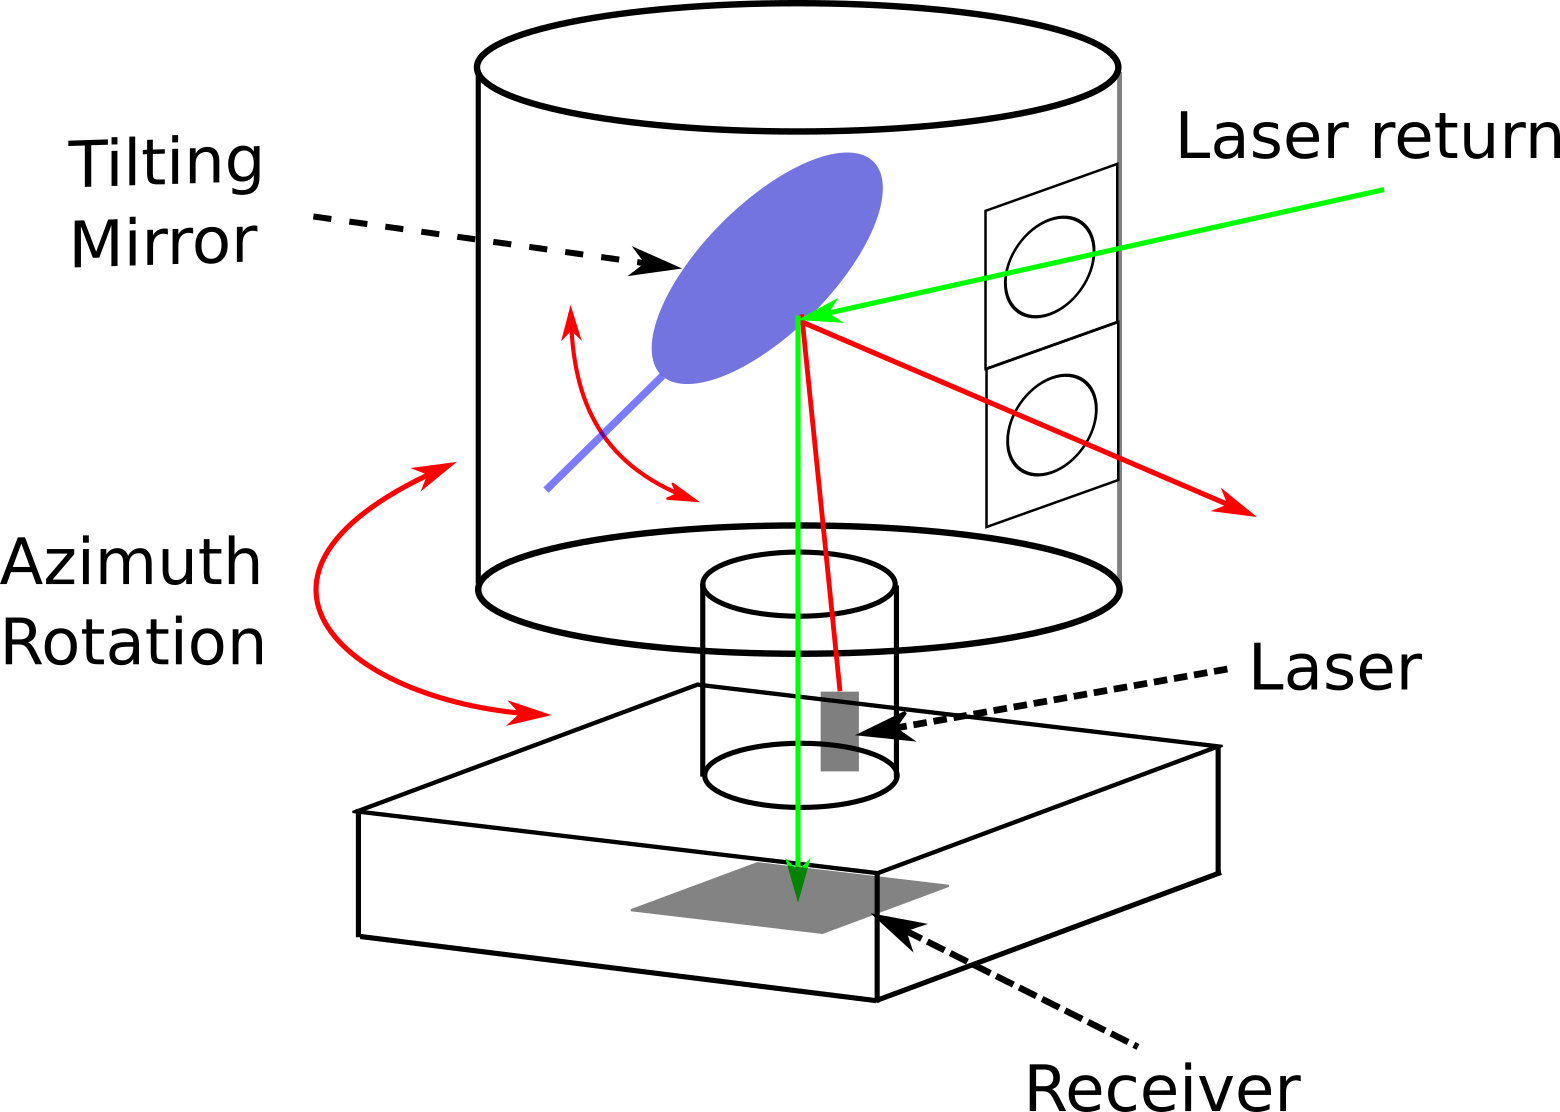
\includegraphics[width=0.5\textwidth]{Lidar.png}
	\caption{Setup of a mechanical spinning \acrshort{lidar} \cite{Li2020}}
	\label{fig:lidar}
\end{figure}
\gls{lidar} is a method to measure distance to objects.
Similar to other systems such as \gls{sonar} or \gls{radar}, \gls{lidar} uses the time-of-flight principle.
A short laser pulse with the velocity $v$ is sent into the environment and the reflected light is analyzed.
The duration $\Delta t$ it took from sending to receiving can then be used to calculate the distance $s$ between the \gls{lidar} and the object that the light hit with
\begin{equation}
	s = c\frac{\Delta t}{2}
\end{equation}
with $c$ being the speed of light.
The change of intensity and wavelength of the returning light are measured as well and can provide information about the reflectivity of the object (intensity) or the chemical composition of the air (wavelength).
Common uses of \gls{lidar} are the analysis of earth's atmosphere, 3D mapping of environments or in the field of autonomous driving for object detection, tracking and \gls{slam}.
Basically all applications which use \gls{radar} can also be used with a \gls{lidar} instead, allowing for a greater accuracy.\\
There are different \gls{lidar} types but their working principles are similar.
A transmitter generates a signal and sends it into the environment using a scanning system and a transmission optic.
As transmitter a laser with a wavelength of \SIrange{850}{950}{\nano\metre} (near-infrared) is typically used.
The scanning system allows the laser to explore a large area instead of only a single point by steering the light at different azimuths and vertical angles and can be divided in mechanical spinning or solid state systems.
Mechanical spinning systems is the oldest technology and is still mainly used today.
A mirror which can be rotated around an axis is used, allowing for a greater vertical \gls{fov}.
Also the whole \gls{lidar} base on which the laser is mounted can be rotated independently from the mirror, allowing for a \SI{360}{\degree} horizontal \gls{fov}.
To get a sufficient resolution the \gls{lidar} has to spin at a high speed, but some \gls{lidar}s also use additionally a vertical array of lasers instead of only one to further increase the density of the generated point cloud.
The working principle of a \gls{lidar} using the mechanical spinning method is shown in figure \ref{fig:lidar}.
While mechanical spinning systems are very precise, they are bulky, need a lot of power and are expensive \cite{Fujii2005}.\\
Solid state systems and especially \gls{mems} \gls{lidar}s try to overcome those problems.
\gls{mems}-\gls{lidar} are quasi-static, the only part that moves is the on the chip embedded mirror, but due to the small size (\SIrange{1}{7}{\milli\metre} diameter) very little power has to be used to move it.
The mirror can be rotated on up to two axes, but because the base cannot be rotated as with mechanical systems, a horizontal view of \SI{360}{\degree} is not possible.
Though by using multiple lasers with different incident angles the \gls{fov} can be increased.
Advantages of \gls{mems}-\gls{lidar}s compared to mechanical systems are the smaller form factor and lower cost \cite{Wang2020}.\\
After transmitting the laser signal the reflected light passes through the receiving optic and is received by photodetectors.
A processing unit then generates a 3D point cloud from all the received measurements.


\subsection{Wheel speed sensor}
The wheel speed sensors measure the speed of each wheel and allow for the calculation of the car velocity.
The measurements are also used by many driver assistance systems such as \gls{abs} to be able to detect wheel slip.
Different techniques exist to measure the speed with the most common ones being magnetoelectric and Hall type wheel speed sensors.\\
The magnetoelectric sensor is composed of a sensor head and a ring gear.
The head is mounted stationary on the car frame while the ring gear is mounted on the wheel hub or axle and rotates with the wheel.
The sensor head is composed of a permanent magnet core and a coil.
When the wheel and thus the ring gear turns the teeth and gaps of the wheel pass by the sensor head and change the magnetic field which induces an alternating voltage in the coil.
The amplitude and frequency of the induced voltage increases with increasing wheel speed.
Advantages of the technique are the low cost, robustness and good performance even in the presence of mud etc.
A disadvantage is the frequency dependency, very low speeds can not be measured due to the induced voltage being too small, while at very high speeds the changes can not be picked anymore up by the head \cite{AutoReif2014}.\\
Nowadays, almost exclusively the hall wheel speed sensor is used.
The functionality is similar to that of the magnetoelectric sensor, but instead of ring gear a ring, on which alternating north and south magnets are placed, is used.
The hall element in the sensor head measures the alternating magnetic field.
A signal amplifier and processing unit is integrated in the sensor head and thus allows for a greater detection rate and range \cite{Re2011}.


\subsection{Camera?}
\itodo{Probably not necessary, as everyone knows what a camera is}



\section{ROS}
\todoin{Brief introduction to ROS}
\gls{ros} is a framework that allows the communication between sensors and actuators of a robot.
It is a meta-operating system and provides services such as hardware abstraction, low-level device control......
Different languages such as C++, Python or Lisp are supported.
The fundamental concepts are nodes, messages, topics and services \cite{Quigley2009}.
A node is a process that performs computation and should be responsible for only one task.
A package can contain multiple nodes.
The communication between nodes is done using messages.
There are different type of messages, but they all consist of standard types such as integer, float or bool but can also contain other messages.
The messages are published on a specific topic.
The topic can then be subscribed by other nodes, to retrieve the messages.
A topic can be published and subscribed by multiple different nodes.
Services allow for a synchronized communication, instead of the asynchronous topics.



\section{Signal processing}
\dots is necessary.
\dots can be divided into filtering and smoothing.
Filtering can be used in live applications and produces an estimate of the current value by taking the past values into account, whereas smoothing uses past and future samples and thus introduces a delay if used on live data \todo{filtering also often introduces a delay}.
Because the detection should be live, only the filtering methods will be examined.
\itodo{How much about dsp? E.g. also noise, aa etc or only type of filters?}
Digital filters can be generally divided into two different categories.
\gls{fir} filter rely on a fixed number of recent input values. An example would be the moving average filter, which takes the past $n$ values into account.
\gls{iir} filter rely on previous output as well as most recent input by summing all points with a certain weight (e.g. exponential filter).
This also explains the naming of the two types, the \gls{fir} filter "forgets" past values, whereas the \gls{iir} filter uses the previous estimate and thus theoretically takes all past values into account.\\
Savitzky-Golay filter
\begin{equation}
	y = \frac{1}{h}\sum_{i =\frac{1 - m}{2}}^{\frac{m - 1}{2}}C
\end{equation}